\section{Specification of the Surface Language}
\label{sec:grammars-and-metamodels:SL-specification}

To define our surface language, we must specify its syntax, semantics, and embedding in the \UML.
The syntax of the surface language and its embedding in the \UML are described below.
The semantics of the language is defined implicitly by describing the transformation from behavior specified in our surface language to \Activities.


\subsection{Syntax}
\label{sub:grammars-and-metamodels:Syntax-SL}

The syntax of behavior modeled in our surface language is defined as follows.
\[
\begin{array}{lcl}
\nonterminal{SLB} & ::= & \terminal{behavior}~\terminalsymbol{\{}~[\nonterminal{MVD}]~\nonterminal{MS}~\terminalsymbol{\}}\\
\nonterminal{MVD} & ::= & \terminal{var}~\nonterminal{VD}~\{\terminalsymbol{;}~\nonterminal{VD}\}~\terminalsymbol{|}\\
\nonterminal{VD} & ::= & \nonterminal{VN}~\terminalsymbol{\mathalpha{:}}~\nonterminal{TN}\\
\nonterminal{MS} & ::= & \nonterminal{S}~\{\terminalsymbol{;}~\nonterminal{S}\},
\end{array}
\]
where the structure of variable names~\nonterminal{VN}, and type names~\nonterminal{TN} is left unspecified.
A description of behavior~\nonterminal{SLB} consists of a sequence of variable declarations~\nonterminal{MVD} and a sequence of statements~\nonterminal{MS}.
A variable declaration~\nonterminal{VD} consists of a variable name and a type name.

The syntax of statements is defined as follows.
\[
\begin{array}{lcl}
\nonterminal{S} & ::= & \terminal{if}~\nonterminal{E}~\terminal{then}~\nonterminal{MS}~\terminal{fi}\\
 & | & \terminal{if}~\nonterminal{E}~\terminal{then}~\nonterminal{MS}~\terminal{else}~\nonterminal{MS}~\terminal{fi}\\
 & | & \terminal{while}~\nonterminal{E}~\terminal{do}~\nonterminal{MS}~\terminal{od}\\
 & | & \terminal{return}~\nonterminal{E}\\
 & | & \nonterminal{SN}~\terminalsymbol{(}~[\nonterminal{ME}]~\terminalsymbol{)}~\terminal{to}~\nonterminal{E}\\
 & | & \nonterminal{E}~\terminalsymbol{.}~\nonterminal{ON}~\terminalsymbol{(}~[\nonterminal{ME}]~\terminalsymbol{)}\\
 & | & \nonterminal{E}~\terminalsymbol{.}~\nonterminal{SFN}~[\terminalsymbol{[}~\nonterminal{N}~\terminalsymbol{]}]~\terminalsymbol{\assignop}~\nonterminal{E}\\
 & | & \nonterminal{VN}~[\terminalsymbol{[}~\nonterminal{N}~\terminalsymbol{]}]~\terminalsymbol{\assignop}~\nonterminal{E},
\end{array}
\]
where the structure of signal names~\nonterminal{SN}, operation names~\nonterminal{ON}, structural feature names~\nonterminal{SFN}, and natural numbers~\nonterminal{N} is left unspecified.
A statement~\nonterminal{S} can contain expressions~\nonterminal{E} and sequences of expressions~\nonterminal{ME}.

The syntax of expressions is defined as follows.
\[
\begin{array}{lcl}
\nonterminal{ME} & ::= & \nonterminal{E}~\{\terminalsymbol{,}~\nonterminal{E}\}\\
\nonterminal{E} & ::= & \terminal{create}~\terminalsymbol{(}~\nonterminal{CN}~\terminalsymbol{)}\\
 & | & \terminal{self}\\
 & | & \nonterminal{VN}\\
 & | & \nonterminal{E}~\terminalsymbol{.}~\nonterminal{SFN}\\
 & | & \nonterminal{E}~\terminalsymbol{.}~\nonterminal{ON}~\terminalsymbol{(}~[\nonterminal{ME}]~\terminalsymbol{)},
\end{array}
\]
where the structure of class names~\nonterminal{CN} and operation names~\nonterminal{ON} is left unspecified.

The note below the class diagram in Figure~\ref{fig:grammars-and-metamodels:UML-diagram-comparison} shows an example of behavior modeled using our surface language.
The behavior is equivalent to the behavior represented by the activity diagram on the left of the figure.

\subsection{Embedding in the UML}
\label{sub:grammars-and-metamodels:UML-embedding}

We use a concept of the \UML called \OpaqueBehavior to embed our surface language in the \UML.
Listing~\ref{lst:grammars-and-metamodels:Embedding-SL} shows a fragment of an XMI representation of a \UML model that contains an instance of \OpaqueBehavior.

\begin{listing}
  \lstset{
    language=xmi,
    label=lst:grammars-and-metamodels:Embedding-SL,
    caption=Embedding in the \UML of behavior modeled using a language called `SL',
    stringstyle=\itshape
  }
  \begin{lstlisting}
    <packagedElement xmi:type="uml:Class" name="C">
      <ownedBehavior xmi:type="uml:OpaqueBehavior" name="b">
        <body>return self</body>
        <language>SL</language>
      </ownedBehavior>
    </packagedElement>
  \end{lstlisting}
\end{listing}

\OpaqueBehavior uses a list of text fragments and a list of language names to specify behavior.
The first list specifies the behavior in one or more textual languages, and the second list specifies which languages are used in the first list.
\OpaqueBehavior can be used to specify behavior using, for instance, fragments of \Java code or natural language.
In our case, as shown in Listing~\ref{lst:grammars-and-metamodels:Embedding-SL}, both lists contain a single item.
The first list contains a specification of behavior using our surface language, and the second list indicates that we use this surface language.

We transform a \UML model containing behavior modeled using our surface language to a \UML model without such behavior by replacing all these occurrences of surface language embedded in \OpaqueBehavior by equivalent \Activities.

\subsection{Transformation}
\label{sub:grammars-and-metamodels:SL-Transformation}

As described in Section~\ref{sub:grammars-and-metamodels:Syntax-SL}, behavior specified using our surface language consists of two parts: a sequence of variable declarations and a sequence of statements.
The process of transforming behavior modeled using a surface language to an \Activity can be divided into two steps:
\begin{enumerate}
\item The variable declarations are translated to \UML \Variables.
\item The sequence of statements is translated to an equivalent group of \ActivityNodes and \ActivityEdges.
\end{enumerate}
Translating variable declarations to \UML \Variables is a trivial step, which we will not discuss.
The transformation of sequences of statements to equivalent fragments of \UML~\Activities is described informally by means of the transformation function~\Transformation{B}.
The function~\Transformation{B} uses the auxiliary transformation functions~\Transformation{MS}, \Transformation{S}, and~\Transformation{E}.

\begin{figure}
\centering
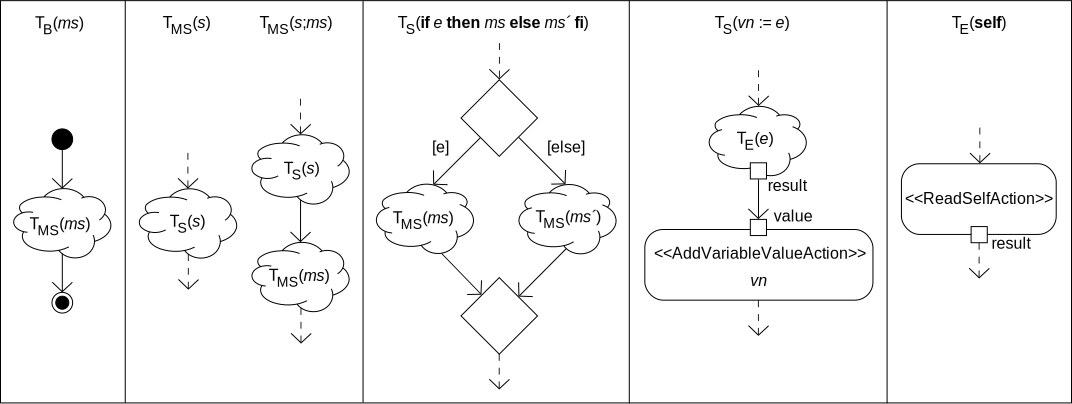
\includegraphics[scale=0.44]{grammars-and-metamodels/figs/transformation}
\caption{Transformations performed by the functions~\Transformation{B}, \Transformation{MS}, \Transformation{S}, and~\Transformation{E}}
\label{fig:grammars-and-metamodels:trans-schematic}
\end{figure}

Figure~\ref{fig:grammars-and-metamodels:trans-schematic} gives a schematic representation of the transformations performed by these functions.
The clouds and the dashed arrows in the figure indicate how the fragments are joined together to create an \Activity.
Each cloud in a fragment is replaced by another fragment of an \Activity.
An incoming dashed \ActivityEdge shows how a fragment is connected to an outgoing \ActivityEdge of the containing fragment; an outgoing dashed \ActivityEdge shows how a fragment is connected to an incoming \ActivityEdge of the containing fragment.

The function~\Transformation{B} creates a group of \ActivityNodes and \ActivityEdges that is equivalent to the sequence of statements provided as input and connects this group with an \InitialNode and an \ActivityFinalNode using two \ControlFlows.
The function~\Transformation{MS} creates an equivalent group of \ActivityNodes and \ActivityEdges for each of the statements in the sequence provided as input and connects these groups using \ControlFlows.
The function~\Transformation{S} creates a group of \ActivityNodes and \ActivityEdges that is equivalent to the statement provided as input.
Statements and expressions that are part of the statement provided as input are also translated to equivalent groups of \ActivityNodes and \ActivityEdges.
These groups are connected to the first group using \ControlFlows, for statements, or \ObjectFlows, for expressions.
The function~\Transformation{E} creates a group of \ActivityNodes and \ActivityEdges that is equivalent to the expression provided as input.
Other expressions that are part of this expression are also translated to equivalent groups of \ActivityNodes and \ActivityEdges.
These groups are connected to the first group using \ObjectFlows. 